\section{Methodology}

\subsection{Literature Survey and Related Work}
The concept of Retrieval-Augmented Generation (RAG) was pioneered to combine the parametric memory of language models with non-parametric external knowledge sources \cite{lewis2020retrieval}. While traditional RAG focuses on textual data, recent studies emphasize multimodal capabilities, bridging textual, visual, and auditory information \cite{radford2021learning}. In the context of secure environments, research highlights the necessity of "local-first" AI. Projects leveraging Ollama and localized transformers have demonstrated that high-parameter models like Llama-3 can be quantized and executed efficiently on consumer-grade hardware without degrading inferential logic. However, comprehensive systems combining local vector databases, UI frameworks, and multimodel execution handlers within an isolated container remain scarce in literature.

\subsection{Existing System Analysis}
Currently deployed systems in secure environments generally fall into two categories:
\begin{enumerate}
    \item \textbf{Rule-Based Offline Searchers:} Traditional enterprise search engines utilizing keyword matching (e.g., Elasticsearch offline deployments). These systems lack semantic understanding and generative summarization capabilities.
    \item \textbf{Isolated Scripts:} Collections of Python scripts running local LLMs. These require extensive command-line knowledge, lack session persistence, and do not offer cohesive multimodal ingestion (processing images and audio alongside text).
\end{enumerate}
\textbf{Limitations:} The primary limitations of existing systems include complex dependency management, lack of semantic visual search, absence of integrated vocal transcription, and a high barrier to entry for end-users operating in high-stress, constrained environments.

\subsection{Proposed System}
The proposed system, Aura, overcomes these limitations by integrating a robust Java Spring Boot backend with local execution sidecars (Python) and a responsive React frontend, all packaged within an Electron desktop shell. Aura provides:
\begin{itemize}
    \item \textbf{Document Processing Engine:} Utilizes Apache PDFBox for local page-by-page text extraction, followed by a managed sliding-window overlapping chunking algorithm.
    \item \textbf{Multimodal Vision and Audio:} Employs a local Hugging Face CLIP model for visual feature extraction and semantic indexing, alongside local Whisper/Vosk Python sidecars for voice transcription, linked seamlessly via Java execution handlers.
    \item \textbf{Grounded Retrieval:} Interfaces with a local Ollama instance running Llama-3 and nomic-embed-text for context-anchored chat generation.
    \item \textbf{Sovereign Vector Storage:} Implements a simulated ChromaDB vector cache mapping utilizing cosine similarity algorithms entirely in memory and persisted to disk, guaranteeing offline functionality.
\end{itemize}

\subsection{System Architecture}
The system architecture of Aura follows a decoupled yet locally integrated micro-monolith approach. The architecture is broadly divided into three tiers: Presentation, Application Logic, and Data/Inference.

\begin{figure}[htbp]
\centering
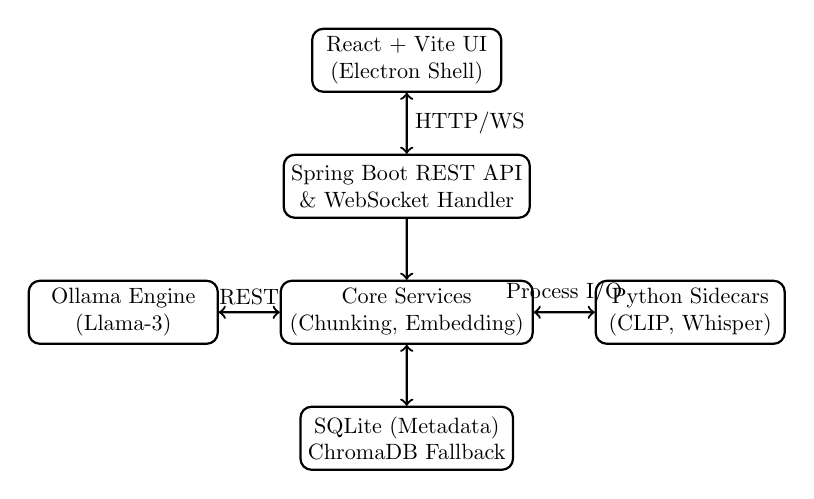
\begin{tikzpicture}[node distance=1.5cm, auto, thick, scale=0.8, transform shape]
    % Nodes
    \node (ui) [draw, rectangle, rounded corners, minimum width=3cm, minimum height=1cm, align=center] {React + Vite UI \\ (Electron Shell)};
    \node (api) [draw, rectangle, rounded corners, minimum width=3cm, minimum height=1cm, below of=ui, node distance=2cm, align=center] {Spring Boot REST API \\ \& WebSocket Handler};
    \node (services) [draw, rectangle, rounded corners, minimum width=4cm, minimum height=1cm, below of=api, node distance=2cm, align=center] {Core Services \\ (Chunking, Embedding)};
    \node (sidecars) [draw, rectangle, rounded corners, minimum width=3cm, minimum height=1cm, right of=services, node distance=4.5cm, align=center] {Python Sidecars \\ (CLIP, Whisper)};
    \node (ollama) [draw, rectangle, rounded corners, minimum width=3cm, minimum height=1cm, left of=services, node distance=4.5cm, align=center] {Ollama Engine \\ (Llama-3)};
    \node (db) [draw, rectangle, rounded corners, minimum width=3cm, minimum height=1cm, below of=services, node distance=2cm, align=center] {SQLite (Metadata) \\ ChromaDB Fallback};

    % Edges
    \draw[<->] (ui) -- (api) node[midway, right] {HTTP/WS};
    \draw[->] (api) -- (services);
    \draw[<->] (services) -- (sidecars) node[midway, above] {Process I/O};
    \draw[<->] (services) -- (ollama) node[midway, above] {REST};
    \draw[<->] (services) -- (db);
\end{tikzpicture}
\caption{Aura Offline Multimodal System Architecture}
\label{fig:architecture}
\end{figure}

\subsection{Security Architecture}
Operating in an air-gapped domain dictates strict security measures. Aura employs:
\begin{itemize}
    \item \textbf{Network Isolation:} The environment variables \texttt{TRANSFORMERS\_OFFLINE=1} and \texttt{HF\_DATASETS\_OFFLINE=1} are explicitly set in Python execution environments to block out-of-band network calls. The backend prevents external IP resolutions during RAG generation.
    \item \textbf{Data Encapsulation:} All vector cache mappings and SQLite databases are stored securely in an isolated application data directory, scrubbed and validated on application boot.
\end{itemize}

\subsection{Algorithms Used}
Aura implements specialized algorithms to ensure contextual accuracy during document ingestion and querying:
\begin{enumerate}
    \item \textbf{Sliding-Window Sentence Chunking:} Defined in the \texttt{ChunkingService}, the algorithm tokenizes extracted text into sentences. It aggregates sentences into chunks up to a defined \texttt{chunk\_size} (e.g., 500 words). To maintain contextual semantic continuity between boundaries, an \texttt{overlap} of sentences (e.g., 100 words) is appended to subsequent chunks.
    \item \textbf{Grounded Generation Pipeline (RAG):} The \texttt{OllamaService} orchestrates the retrieval flow. User queries are vectorized via nomic-embed-text. The vector is compared against the local ChromaDB semantic cache using \texttt{cosineSimilarity}. The top-k highest scoring chunks are appended to the system prompt as contextual groundings. Llama-3 is then instructed via a strict system prompt to formulate an answer strictly from the provided context, rendering source citations alongside the generative stream.
\end{enumerate}
